%=============================================================================
\documentclass[10pt,a4paper]{article}
%
\input{dd4hep-setup.tex}
%
\pagestyle{fancyplain}{\fancyfoot[C]{\sffamily{Software Design of the Alignment 
Extension of the dd4hep Detector Description Toolkit\\
}}}
%
\begin{document}   
%
\mytitle{
DDAlign
\vspace{-0.5cm}
}{
Alignment Support for the \\
\vspace{0.5cm}
dd4hep Geometry Description \\
\vspace{0.5cm}
Toolkit
}
{
\vspace{-2cm}
{\bf\large{Design Document}}\\
\vspace{1cm}
M. Frank \\
{CERN, 1211 Geneva 23, Switzerland}


}  % End of title
%
%==  Abstract  ===============================================================
\pagestyle{plain}
\pagenumbering{Roman}
\setcounter{page}{1}
\begin{abstract}
%=============================================================================

\noindent
\normalsize
Experimental setups in High Energy Physics are highly complex assemblies 
consisting of various detector devices typically called {\it{subdetectors}}.
Contrary to the ideal world, where all these components are of perfect shape 
and at exact positions, existing devices have imperfections both in their 
shape and their relative and absolute positions. These are described by the
alignment parameters.\\
To still measure the detector response from particle collisions with the highest
possible precision, these imperfections are taken into account when converting
measured signals to space-points in the measurement devices. This procedure
is called {\it{detector alignment}}. \DDhep does not want to solve the exact 
problem of the detector alignment itself, but rather support firstly algorithms 
determining the alignment parameters and secondly support the application which 
apply the measured alignment parameters and apply them to the ideal geometry 
for further event data processing.\\
This document describes how \DDhep detector description will accomplish 
the support for detector alignment data structures, how they will be required
by alignment procedures.
The design is strongly driven by easy of use;
developers of detector descriptions and applications using
them should provide minimal information and minimal specific
code to achieve the desired result.

\end{abstract}

\vspace{8cm}

\begin{center}
{\large{\bf{
\begin{tabular} {| l | l | l |}
\hline
\multicolumn{3}{| c |}{} \\[0.2cm]
\multicolumn{3}{| c |}{Document History} \\[0.2cm]
\multicolumn{3}{| c |}{} \\[0.2cm]
\hline
                 &      &        \\
Document         &      &        \\
version          & Date & Author \\[0.2cm] \hline
                 &      &        \\
1.0              & 01/03/2016 & Markus Frank CERN/LHCb  \\
1.1              & 30/06/2016 & Markus Frank CERN/LHCb  \\
                 &            & Revised by workgroup    \\
                 &      &        \\        \hline 
\end{tabular}
}}}
\end{center}

\clearpage
%
%
%==  TOC  ====================================================================
\tableofcontents
\clearpage
%
%
%=============================================================================
% Manual
%=============================================================================
\pagenumbering{arabic}
\setcounter{page}{1}

%=============================================================================
\section{Introduction}
\label{sec:ddalign-user-manual-introduction}
%=============================================================================
\noindent
This manual should introduce to the \DDA framework. 
One goal of \DDA is to easily model geometrical imperfections applied to
the ideal geometry of detection devices as they are typically used in 
high energy physics experiments.

\noindent
To avoid confusion within this document, a few terms need to be defined
with respect to detector alignment:
\begin{itemize}\itemcompact
\item The {\it{ideal geometry}} describes the detector as it was designed.
    Such a detector is an utopic object, which can never be realized in terms
    of the placement of the individual components as such.
\item The {\it{actual geometry}} describes the real detector in the configuration at
    a given time. This includes all the changes i.e. {\it{deltas}} to the 
    {\it{ideal}} geometry. These changes are also called the 
    {\it{alignment parameters}}. These parameters typically are only valid 
    for a defined time interval.
\item {\it{Realignment}} defines the procedure to apply a new set of
    temporary {\it{misalignment parameters}} to the ideal geometry. Such a procedure
    is applied, if a previously applied set of parameters is no longer valid with
    respect to the event data to be processed. In short {\it{realignment}}
    is necessary if the {\it{actual geometry}} of the detector is time dependent.
\end{itemize}

\noindent
\DDA formalizes both the access and the application of alignment parameters 
to the ideal geometry. The possibility to properly describe actual geometries 
with respect to ideal geometries is essential to understand the detector response
to particle collisions and to connect response of geometrical independent
areas of the experiment e.g. to one single track.

\noindent
In this manual we will shortly describe the model used
to describe an experiments detector description and then in more detail 
document the support for alignment with its programming interfaces.

%=============================================================================
\begin{figure}[h]
  \begin{center}
    \includegraphics[height=90mm] {dd4hep_classes.png}
    \caption{Class diagram with the main classes and their relations 
             for the Generic Detector Description Model. The implementing
             ROOT classes are shown in brackets.}
    \label{fig:dd4hep-detector-model}
  \end{center}
\end{figure}
\vspace{-0.1cm}
%=============================================================================
\subsection{Generic Detector Description Model}
\label{subsec:generic-model}
%=============================================================================

\noindent
This is the heart of the dd4hep detector description toolkit. Its purpose is 
to build in memory a model of the detector including its geometrical aspects
as well as structural and functional aspects. The design reuses the elements 
from the ROOT geometry package and extends them in case required functionality 
is not available. Figure~\ref{fig:dd4hep-detector-model} illustrates the main
players and their relationships~\cite{bib:dd4hep}.
Any detector is modeled as a tree of $Detector$ $Elements$, the entity 
central to this design, which is represented in the implementation by 
the $DetElement$ class~\cite{bib:LHCb-geometry}. It offers all
applications a natural entry point to any detector part of the experiment
and represents a complete sub-detector (e.g. TPC), a part of a 
sub-detector (e.g. TPC-Endcap), a detector module or any other convenient 
detector device. 
The main purpose is to give access to the data associated 
to the detector device. For example, if the user writes some TPC reconstruction 
code, accessing the TPC detector element from this code will provide access 
the all TPC geometrical dimensions, the alignment and calibration constants 
and other slow varying conditions such as the gas pressure, end-plate 
temperatures etc. The $Detector$ $Element$ acts as a data concentrator. 
Applications may access the full experiment geometry and all connected data
through a singleton object called $Detector$, which provides 
management, bookkeeping and ownership to the model instances.

\noindent
The geometry is implemented using the ROOT geometry classes, which are used
directly without unnecessary interfaces to isolate the end-user from the 
actual ROOT based implementation.
\DDA allows client to access, manage and apply alignment parameters or 
smallish changes to the ideal geometry. The mechanism to achieve this 
is described in the following.

%=============================================================================
\begin{figure}[h]
  \begin{center}
    \includegraphics[height=75mm] {dd4hep_detelement_tree.png}
    \caption{The object diagram of a hypothetical TPC detector showing in
    parallel the $Detector$ $Element$ and the $Geometry$ hierarchy and the 
    relationships between the objects.}
    \label{fig:dd4hep-hierarchies}
  \end{center}
  \vspace{-0.5cm}
\end{figure}
%=============================================================================
\subsection{Detector Element Tree and the Geometry Hierarchy}
\label{subsect:detelement-hierarchy}
%=============================================================================
\noindent
The geometry part of the detector description is delegated to the ROOT classes.
$Logical$ $Volumes$ are the basic objects used in building the geometrical hierarchy. 
A $Logical$ $Volume$ is a shape with its dimensions and consist of a given material. 
They represent unpositioned objects which store all information about 
the placement of possibly embedded volumes. The same
volume can be replicated several times in the geometry. The $Logical$ $Volume$ also 
represents a system of reference with respect to its containing volumes.
The reuse of instances of $Logical$ $Volumes$ for different placements 
optimizes the memory consumption and detailed geometries for complex setups
consisting of millions of volumes may be realized with reasonable amount of memory.
The difficulty is to identify a given positioned volume 
in space and e.g. apply alignment parameters to one of these volumes. 
The relationship between the Detector Element and the placements
is not defined by a single reference to the placement, but the full path 
from the top of the detector geometry model to resolve existing
ambiguities due to the reuse of $Logical$ $Volumes$.
Hence, individual volumes must be identified by their full path from mother 
to daughter starting from the top-level volume. 

\noindent
The tree structure of
$Detector$ $Elements$ is a parallel structure to the geometrical hierarchy.
This structure will probably not be as deep as the geometrical one since 
there would not need to associate detector information at very fine-grain 
level - it is unlikely that every little metallic screw
needs associated detector information such as alignment, conditions, etc.
Though this screw and many other replicas must be described in the geometry 
description since it may be important e.g. for its material contribution 
in the simulation application. Thus, the tree of Detector Elements is
fully degenerate and each detector element object will be placed only 
once in the detector element tree as illustrated for a hypothetical
Time Projection Chamber (TPC) detector in 
Figure~\ref{fig:dd4hep-hierarchies} with an ideal geometry,
where no positioning corrections are applied to neither child. It is essential to 
realize that the geometry tree in an ideal geometry is degenerate contrary 
to the tree of detector elements.

\noindent
It should be noted, that alignment parameters may be applied to any volume 
of the ideal geometry. The alignment only affects the actual position of 
a volume it is e.g. irrelevant if the volume is sensitive or not.

%=============================================================================
\begin{figure}[h]
  \begin{center}
    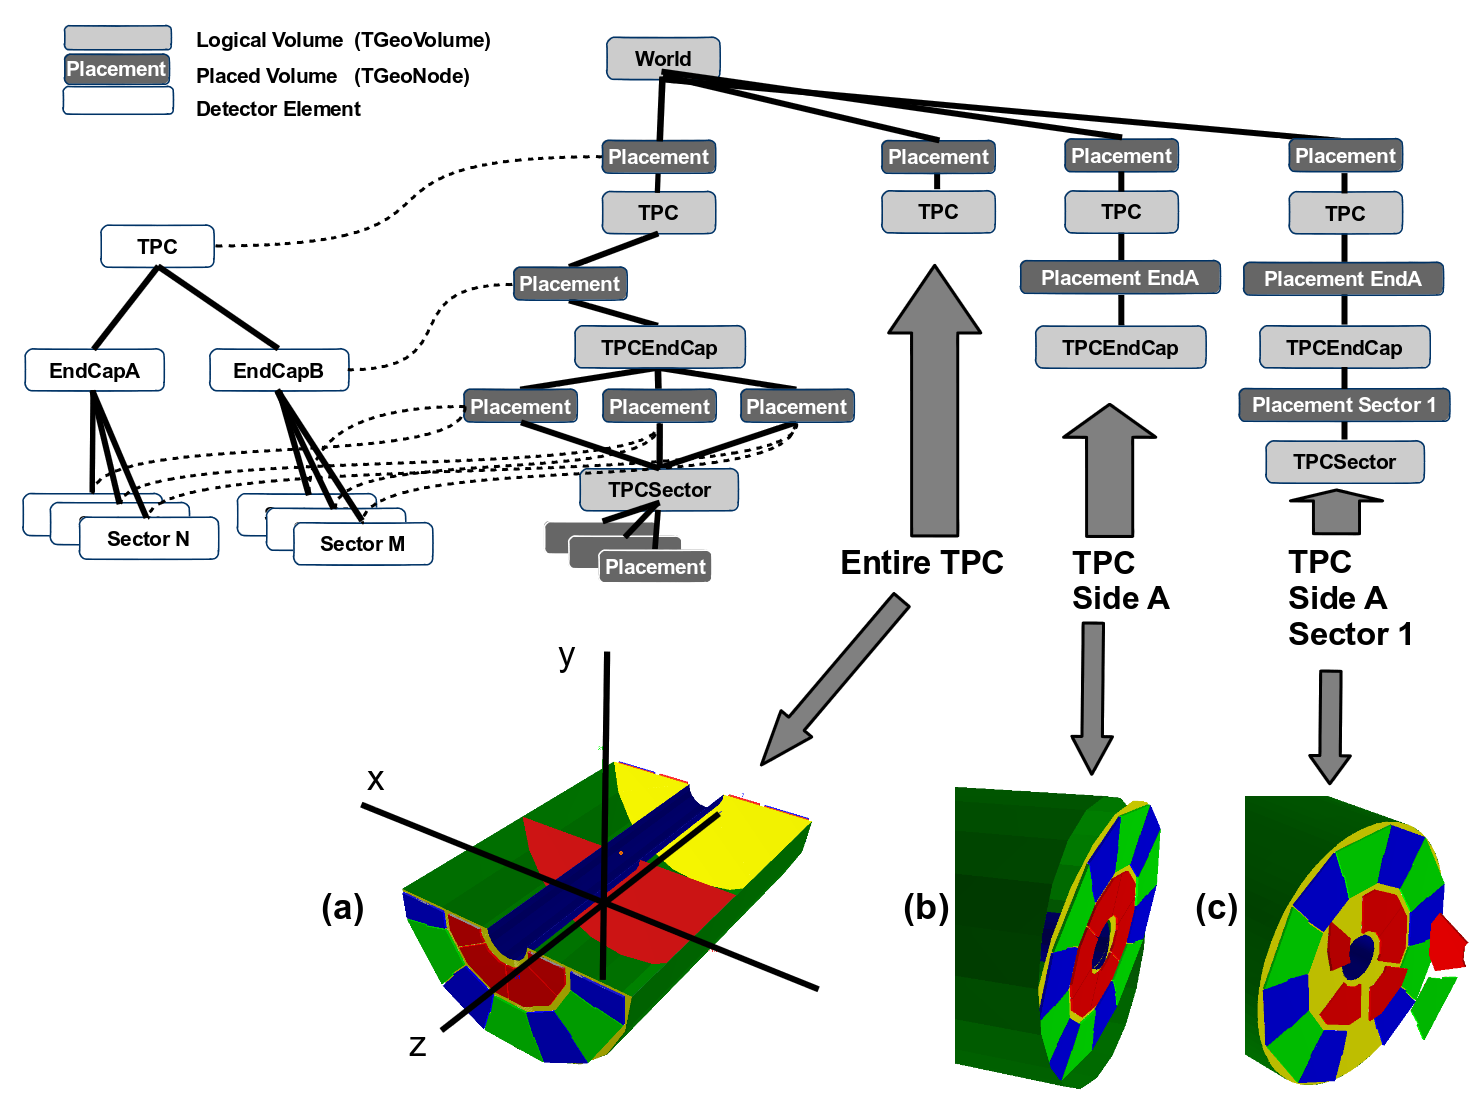
\includegraphics[width=160mm] {DDAlign_detelement_aligned_tree.png}
    \caption{The object diagram of a hypothetical TPC detector showing in
    parallel the $Detector$ $Element$ and the $Geometry$ hierarchy and examples
    of mispositioned detector parts: (a) mispositioned entire subdetector 
    (translation), (b) mispositioned end-cap (tilt) and (c) mispositioned
    individual sectors within one endcap.}
    \label{fig:dd4hep-aligned-hierarchies}
  \end{center}
\end{figure}
%=============================================================================
\subsection{Alignment Parameters of Detector Components}
\label{subsect:ddalign-intro-aligments}
%=============================================================================
\noindent
Alignment parameters never apply in the same way to {\it{all}} placements of the 
same volume in this hierarchy. Hence, to (re-)align a volume in the hierarchy
means to lift a full branch of placements from the top volume down to
the element to be (re-)aligned out of this shared hierarchy and apply
a correction matrix to the last node. This procedure is illustrated in 
Figure~\ref{fig:dd4hep-aligned-hierarchies}. Re-alignment of volumes may occur
at any level. In the above example of a TPC this results in the following effects:

\noindent
\begin{itemize}\itemcompact
\item A realignment of the entire subdetector, i.e. the TPC as a whole, 
    would affect consequently move all contained children with respect to the 
    top level coordinate system. An example is shown in 
    Figure~\ref{fig:dd4hep-aligned-hierarchies} (a). A movement of the subdetector
    would affect all transformation between local coordinates of any part of the
    subdetector to the top level coordinate system. Such effects would be visible 
    at all stages of the data processing e.g. when translating signals from 
    particles into global coordinates.
\item A realignment of parts of a subdetector affects only the partial subdetector
    itself and child volumes at lower levels. As in the example, where the entire
    subdetector is moved, here only the sectors on one side of the TPC would be affected
    as shown in Figure~\ref{fig:dd4hep-aligned-hierarchies} (b).
\item In Figure~\ref{fig:dd4hep-aligned-hierarchies} (c) within one end-cap of the TPC
    individual sectors may not be positioned at the ideal location
    (Figure~\ref{fig:dd4hep-aligned-hierarchies} (c) exaggerates: 
    ''flying sectors'' are a rather rare case in reality).
    Finally also the sectors itself could be fragmented and be assemblies of other
    shapes, which are not ideally placed and may need correction.
\end{itemize}
The origin of the volume misplacements may be many-fold:
\begin{itemize}\itemcompact
\item Elements may be weak and assembled parts move due to weak support structures.
    This is a common problem e.g. for tracking detectors, where heavy and solid 
    structures dramatically influence the measurement result~\footnote{Clearly the 
    alignment mechanism is not limited to tracking detectors, but rather valid 
    for any volume used to describe the detector.}.
    Misplaced sectors could e.g. be the consequence of a deforming end-cap frame due 
    to the weight of the sectors.
\item Environmental conditions such as the temperature may influence the 
    position or the shape of a volume.
\item Some of the measurement equipment may be moved from a parking position into 
    a data taking position such as the two halves of the LHCb vertex detector. 
    Whereas the position of the sensors on each half are known to a very high 
    precision, the position of the absolute position of the two halves with respect
    to the full experiment may change after each movement.
\end{itemize}
Changes to the volume placement do not only affect sensitive material i.e. detector
components with an active readout, but also passive material. The placement 
of any volume, passive or active, may be corrected using \DDA. The determination
of the alignment parameters of passive components however may be more difficult 
in the absence of located signals resulting e.g. from the traversal of a track.

\noindent
All effects resulting from such causes obviously need to be corrected in order to 
fully explore the capabilities of the detection devices and to minimize 
measurement errors. In general any deviation from the ideal position of a volume
can be described by two elementary transformations:
\begin{itemize}\itemcompact
\item a translation
\item a rotation around a pivot point.
\end{itemize}
giving a full transformation matrix of the form:
\begin{equation}
T = L * P * R * P^{-1}
\end{equation}
where 
\begin{itemize}\itemcompact
\item $T$ is the full transformation in 3D space containing the change to the 
exiting placement transformation. The existing placement is the placement 
transformation of the volume with respect to the mother volume.
\item $L$ is a translation specifying the position change with respect to the 
    mother volume.
\item $P * R * P^{-1}$ describes a rotation around a pivot point specified 
    int he mother volume's coordinate system.
\item $P$ is the translation vector from the mother volumes origin to the 
    pivot point. The concept of a pivot point does not introduce a new set of
    parameters. Pivot points only help to increase the numerical precision.
\end{itemize}
Most of the changes do not require the full set of parameters. Very often 
the changes only require the application of only a translation, only a rotation
or both with a pivot point in the origin. These simplifications are supported 
in the user interface described in 
Section~\ref{sec:ddalign-user-manual-ddalign-interface}.

%=============================================================================
\begin{figure}[t]
  \begin{center}
    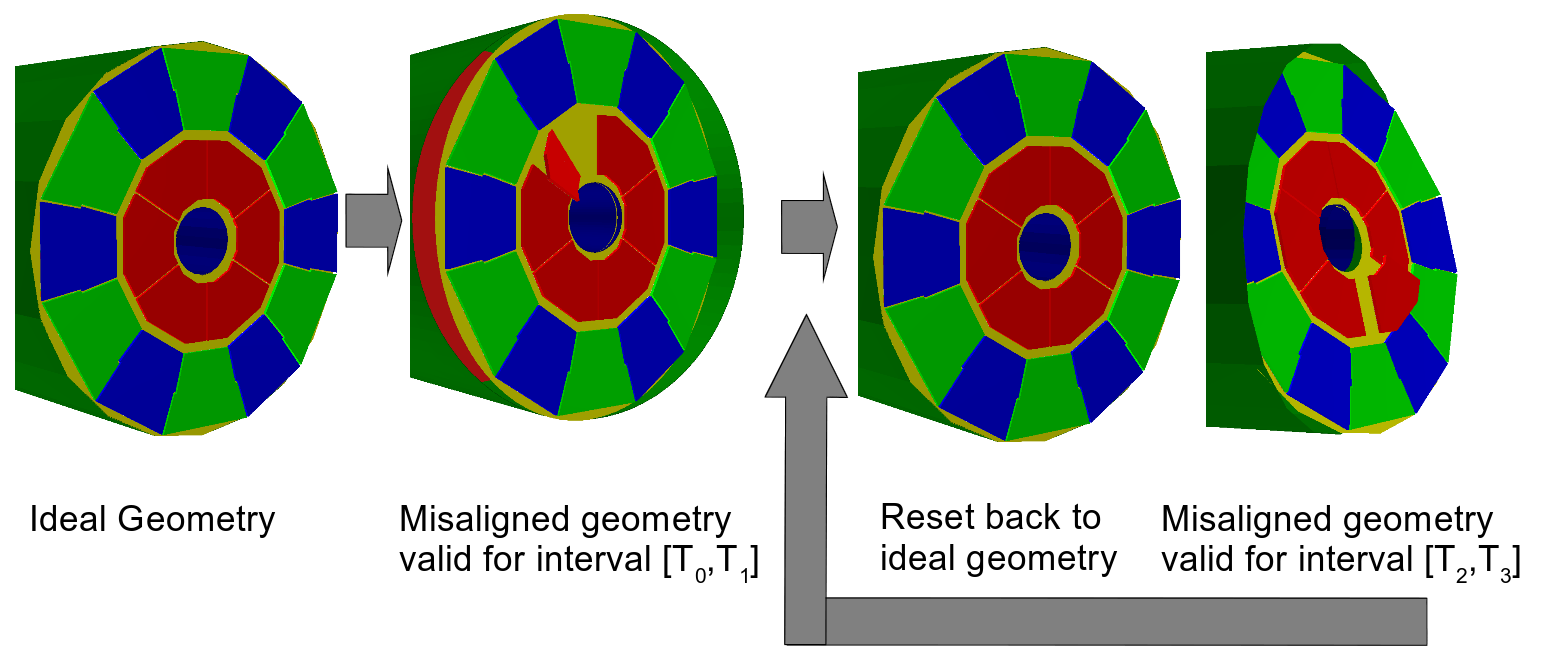
\includegraphics[width=160mm] {DDAlign-iterative-misalignment.png}
    \caption{The iterative application of alignment parameters as described
    in Section~\ref{subsect:ddalign-intro-iterative-alignments}.
    For each interval of validity ($[T_0,T_1]$, $[T_2,T_3]$, $[T_4,T_5]$, ...)
    a seperate set of alignment constants is applied to the ideal geometry.
    The two steps to reset the misaligned geometry back to the ideal geometry and
    to re-apply a new set of alignment constants may be executed as 
    often as necessary when processing data from particle collisions.}
    \label{fig:ddalign-aligned-iterative}
  \end{center}
\end{figure}

%=============================================================================
\subsection{Iterative Application of Alignments}
\label{subsect:ddalign-intro-iterative-alignments}
%=============================================================================
\noindent
In the general case a given set of alignment parameters is not static and 
may very well change with time. For this reason it is highly important to 
support not only one single realignment step.
Hence, the following scenario is an important use case:
\begin{enumerate}\itemcompact
\item Create the ideal detector using an ideal geometry.
\item Apply a set of alignment parameters for a given time 
    interval corresponding to the 
    time a set of particle collisions were collected in the experiment.
\item Process the set of collected particle collisions.
\item Reset the misaligned detector to the ideal.
\item Choose new event data input corresponding to another time interval
    and restart at item 2.
\end{enumerate}
Graphically this use case is illustrated in 
Figure~\ref{fig:ddalign-aligned-iterative}. In 
Section~\ref{sec:ddalign-user-manual-ddalign-interface} the implementation 
to realize this use case is described.

%=============================================================================
\subsection{Procedures to Determine Alignment Parameters}
\label{subsect:ddalign-intro-determine-alignment-params}
%=============================================================================
\noindent
Typically the determination of alignment parameters requires a starting point
which is not necessarily identical to the ideal position of a 
volume~\cite{bib:chris-parkes-priv-comm}. These volume positions are the result
of a survey measurement or the result of internal position measurements 
of a sub-volume within a sub-detector e.g. on a measurement bench.
In the following we call these parameters {\it{survey parameters}}. 
{\it{Survey parameters}} default to the ideal volume position if not supplied,
alternatively, if set, to the provided position. {\it{Survey parameters}}
are, like the alignment parameters, provided in terms of {\it{changes}} with 
respect to the ideal position and hence may be treated in a similar way.

\noindent 
The survey parameters are - like alignment parameters - accessible to users
through the interface offered by the $DetElement$ objects.

%=============================================================================
\subsection{Simulation of Non-Ideal, Real Detector Geometries}
\label{subsect:ddalign-intro-simulate-misaligned-geometries}
%=============================================================================
\noindent
It is a standard procedure in high energy physics to at least verify 
the measured detector response of a given physics process in particle 
collisions with the expected simulated detector response.
For most purposes the simulation of an ideal detector is certainly is
sufficient - though not describing the full truth. Sometimes however, the
detector geometry must be simulated with a geometry as close to the 
known geometry as possible.

\noindent
The simulation of such a geometry with applied alignment parameters can 
rather easily be realized using using the \DDhep, \DDA and the \DDG frameworks:
\begin{itemize}\itemcompact
\item The ideal geometry is constructed using the standard procedures
    of \DDhep\cite{bib:dd4hep}.
\item Then the alignment parameters are applied.
\item Finally the corrected geometry is translated to $Geant4$~\cite{bib:geant4}
    using the \DDG\cite{bib:DDG4} package.
    All particle collisions simulated with this translated geometry 
    correspond to the modified geometry including the geometry modifications.
\end{itemize}

\noindent
There is a caveat though: The application of alignment parameters can
easily create volume overlaps, which are highly disliked by the $Geant4$ 
runtime. If the above described procedure is applied, it is highly advised 
to check the resulting geometry for overlaps. Both, $ROOT$~\cite{bib:ROOT-tgeo}
and $Geant4$~\cite{bib:geant4} offer tools to perform such tests.

\noindent
Simulating displaced geometries was typically not supported by most toolkits
in the past. \DDA can offer this feature due to the feature of the $ROOT$ 
geometry toolkit, which actually replaces individual branches of the 
geometry with truly new placements.


%=============================================================================
\subsection{Alignment Constants in Multi-Threaded Data Analysis}
\label{subsect:ddalign-intro-multi-threading}
%=============================================================================
\noindent
Once alignment constants are applied, the \DDhep geometry is read-only.
Read-only data structures are by definition thread safe. Multiple threads
processing events in parallel will not cause race conditions as long as 
all events processed in parallel require the same alignment constants.
Race conditions may only appear in the event new alignment constants must be 
applied e.g. when the conditions between subsequent events change.

\noindent
It is assumed that the hosting framework supports the required actions
necessary:
\begin{itemize}\itemcompact
\item Drain the event queue
\item Apply the new alignment constants
\item Re-enable the flow of events to be processed.
\end{itemize}
\noindent
Though this is not the only way how to handle multi-threading issues, for
data analysis and reconstruction this mechanism is the current baseline
unless new requirements emerge from new use-cases of clients.


\newpage
%=============================================================================
\section{The Envisaged DDAlign User Interface}
\label{sec:ddalign-user-manual-ddalign-interface}
%=============================================================================

\noindent
\DDA implements a machinery to apply and access the alignment parameters
describing the difference between an ideal detector given by an ideal geometry
and the geometry of the actually built assembly in real life.
To ease its usage for the clients and to shield clients from the 
internals when actually dealing with realigned geometries, a set of 
helper classes was designed. The access to the alignment parameters 
in read-only mode was separated from the import or export thereof.

\noindent
As a basic concept within \DDhep any {\it{sizable}} detector component
can be realigned. {\it{Sizable}} as a rule of thumb is anything, which 
is manufactured as an individual piece and which you may ''hold in your hands''.
Such objects are also described by a $detector$ $element$ of type {\tt DetElement}.
An example is e.g. a single silicon wafer of a tracking device or the entire
tracking detector itself.
The access to the alignment parameters is possible from each {\tt DetElement}
instance as described in Section~\ref{sec:ddalign-user-manual-misalignment-access}.
The interface assumes ''planar'' alignment parameters i.e. the shape of 
a given volume does not change~\footnote{This is a restriction to the 
possibilities provided by the ROOT implemetation~\cite{bib:ROOT-tgeo}
based on experience~\cite{bib:chris-parkes-priv-comm}.
If at a later time the need arises the provided alignment interface may 
be extended to support shape changes.}.

\noindent
Please be aware that the extensive use of misalignments is highly memory
consuming.

\noindent
%=============================================================================
\subsection{Access to Alignment Parameters from the Detector Element}
\label{sec:ddalign-user-manual-misalignment-access}
%=============================================================================

\noindent
The $DetElement$ class as shown in Figure~\ref{fig:dd4hep-detector-model}
gives the user access to the alignment structure of type $Alignment$ as 
illustrated in the following example:
\begin{code}
    DetElement wafer = ... // Valid handle to a detector element
    Alignment  wafer_alignment = wafer.alignment();
    if ( wafer_alignment.isValid() )  {
        // This wafer's placement differs from the ideal geometry when
        // alignment parameters are present.
        
        // Access the misalignment transformation with respect to the parent volume:
        Transform3D tr = wafer_alignment.toMotherDelta();
    }
\end{code}
The access to details of an invalid alignment object results in a runtime 
exception. The following calls allow clients to access alignment information
from the $DetElement$ structure:
\begin{code}
      /// Access to the actual alignment information
      Alignment alignment() const;

      /// Access to the survey alignment information
      Alignment surveyAlignment() const;
\end{code}
The call to $alignment()$ return the parameters $applied$ to the the existing
ideal geometry. The call $surveyAlignment()$ returns optional constants used 
to perform numerical calculations as described in 
section~\ref{subsect:ddalign-intro-determine-alignment-params}.

\noindent
All functionality of the DetElement, which depends on applied alignment parameters
are automatically updated in the event of changes. These are the geometry 
transformations with respect to the mother- and the world volume:
\begin{code}
      /// Create cached matrix to transform to world coordinates
      const TGeoHMatrix& worldTransformation() const;

      /// Create cached matrix to transform to parent coordinates
      const TGeoHMatrix& parentTransformation() const;
 
      /// Transformation from local coordinates of the placed volume to the world system
      bool localToWorld(const Position& local, Position& global) const;

      /// Transformation from local coordinates of the placed volume to the parent system
      bool localToParent(const Position& local, Position& parent) const;

      /// Transformation from world coordinates of the local placed volume coordinates
      bool worldToLocal(const Position& global, Position& local) const;

      /// Transformation from world coordinates of the local placed volume coordinates
      bool parentToLocal(const Position& parent, Position& local) const;
\end{code}
it is worth noting that the update of cached information is performed by the $DetElement$ 
objects, other user defined cached information is {\bf{not}} updated. Such a mechanism
shall be provided using update callbacks, which have to be registered to individual 
$DetElement$ entities.

\noindent
The interface of the $Alignment$ structure to access detector 
alignment parameters is as follows (see also the corresponding header file dd4hep/Alignment.h):
\begin{code}
      /// Number of nodes in this branch (=depth of the placement hierarchy from the top level volume)
      int numNodes() const;
      
      /// Access the placement of this node
      PlacedVolume placement()   const;
      /// Access the placement of the mother of this node
      PlacedVolume motherPlacement(int level_up = 1)   const;

      /// Access the placement of a node in the chain of placements for this branch
      PlacedVolume nodePlacement(int level=-1)   const;

      /// Access the currently applied alignment/placement matrix with respect to the world
      Transform3D toGlobal(int level=-1) const;
      /// Transform a point from local coordinates of a given level to global coordinates
      Position toGlobal(const Position& localPoint, int level=-1) const;
      /// Transform a point from global coordinates to local coordinates of a given level
      Position globalToLocal(const Position& globalPoint, int level=-1) const;

      /// Access the currently applied alignment/placement matrix with respect to mother volume
      Transform3D toMother(int level=-1) const;

      /// Access the currently applied alignment/placement matrix (mother to daughter)
      Transform3D nominal() const;

      /// Access the currently applied correction matrix (delta) (mother to daughter)
      Transform3D delta() const;

      /// Access the inverse of the currently applied correction matrix (delta) (mother to daughter)
      Transform3D invDelta() const;
\end{code}

\begin{itemize}\itemcompact
\item The calls in line 3-7 allow access to the relative position of the $nth.$ element
    in the alignment stack with respect to its next level parent. 
    Element $numNodes()-1$ denotes the lowest level and element $0$ is the world 
    volume. The default argument $(-1)$ addresses the lowest placement in the hierarchy.
\item Calls in line 9-10 allow to access/execute transformations from a given level
    in the placement hierarchy to coordinates in the top level volume (world).
\item The call in line 13 allows to transform a global coordinate to the local coordinate
    system in a given level of the hierarchy. The other two calls of this block support
    coordinate transformations between local and global coordinate systems.
\item The call $toMother$ in line 20 returns the local transformation of the node at
    a given level to the mother's coordinate system.
\item The calls in line 16-20 give access to the nominal placement matrix of the realigned
    node with respect to the parent volume and the changes thereof.
\end{itemize}
Besides these convenience calls the full interface to the class {\tt TGeoPhysicalNode}, 
which implements in the ROOT geometry package the support for alignment changes 
is accessible from the $Alignment$ object handle.
Further documentation is available from the \tgeo{TGeoPhysicalNode}{ROOT documentation}.

\noindent
%=============================================================================
\subsection{Manipulation of Alignment Parameters}
\label{sec:ddalign-user-manual-misalignment-manip}
%=============================================================================
There are multiple possibilities to apply alignment parameters:
\begin{itemize}\itemcompact
\item The pedestrian way ''by hand'' using C++ as described in 
    Subsection~\ref{sec:ddalign-user-manual-misalignment-manip-cxx}
\item Loading a whole set of misalignment constants from XML, the ''poor man's'' database.
    This mechanism is described in
    Subsection~\ref{sec:ddalign-user-manual-misalignment-manip-xml}
\item Loading a whole set of misalignment constants from a database.
    This possibility depends heavily on the database and its schema used.
    A typical use case is to load misalignment constants depending on the
    experiment conditions at the time the event data were collected.
    \DDA does not provide an implementation.
    This possibility here is only mentioned for completeness and will be subject 
    to further developments to support conditions in \DDhep. 
\end{itemize}


\newpage
%=============================================================================
\begin{thebibliography}{9}
\bibitem{bib:dd4hep} M. Frank et al, "dd4hep: A Detector Description Toolkit 
                for High Energy Physics Experiments",
                detailtional Conference on Computing in High Energy and Nuclear Physics  
                (CHEP 2013), \\
                Amsterdam, Netherlands, 2013, proceedings.

\bibitem{bib:LHCb-geometry} S. Ponce et al., 
                "Detector Description Framework in LHCb", 
                detailtional Conference on Computing in High Energy and Nuclear Physics  (CHEP 2003), 
                La Jolla, CA, 2003, proceedings. 
\bibitem{bib:chris-parkes-priv-comm} C. Parkes, private communications.
\bibitem{bib:DDG4} M.Frank, "DDG4 - A Simulation Toolkit for High Energy 
                Physics Experiments using Geant4 \\
                and the dd4hep Geometry Description".
\bibitem{bib:ROOT-tgeo} R.Brun, A.Gheata, M.Gheata, "The ROOT geometry package",\\
                    Nuclear Instruments and Methods {\bf{A}} 502 (2003) 676-680.
\bibitem{bib:geant4}  S. Agostinelli et al., 
                   "Geant4 - A Simulation Toolkit", \\
                    Nuclear Instruments and Methods {\bf{A}} 506 (2003) 250-303.

\end{thebibliography}
%=============================================================================
\end{document}
